\begin{figure}[H]
    \setlength{\abovecaptionskip}{2pt}
    \setlength{\belowcaptionskip}{2pt}
    \centering
    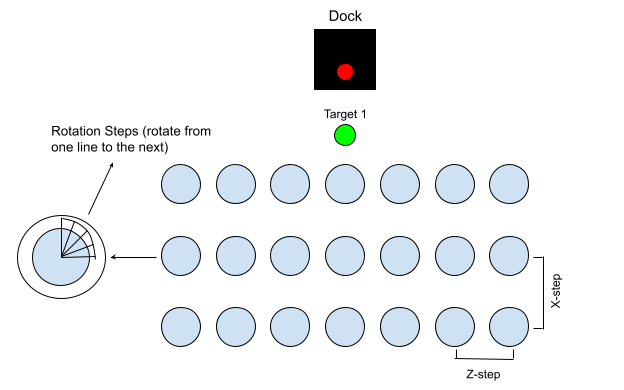
\includegraphics[width=\linewidth]{figures/src/data_camera_movement_algo.png}
    \caption{
	    \textbf{Data Camera Movement Procedure} Our data camera moves in z-steps and x-steps, with rotations for each z-step. We obtain an image with each rotation step. 
    }
    \label{fig:data_camera_movement_algo}
\end{figure}
